\section{Background}


\cite{xray}


\subsection{Kiessig fringes}

\begin{figure}
	\centering
	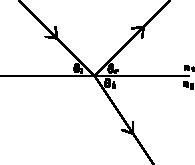
\includegraphics[width=0.33\textwidth]{content/graphics/fresnel.pdf}
	\caption{Depiction of reflection and refraction of light rays on a smooth surface.}
	\label{fig:fresnel}
\end{figure}

Fresnel's formulae\footnote{Followin the derivation in \cite{idfk} among others.}

\cite{Kiessig_1931}

\begin{figure}
	\centering
	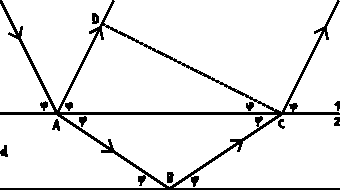
\includegraphics[width=0.55\textwidth]{content/graphics/kiessig.pdf}
	\caption{Schematic light paths in systems of a thin layer on a substrate responsible for Kiessig oscillations according to \cite{Kiessig_1931}.}
	\label{fig:kiessig}
\end{figure}


\subsection{Stratified media}

\cite{Parratt_1954}

\begin{figure}
	\centering
	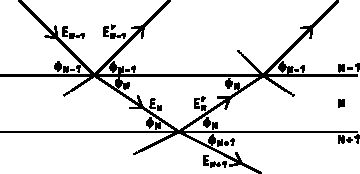
\includegraphics[width=0.66\textwidth]{content/graphics/parratt.pdf}
	\caption{Conceptual visualization of the Parratt algorithm presented in \cite{Parratt_1954}.}
	\label{fig:parratt}
\end{figure}
